\scanpage{4}
% Archive foliation: 3, lower right. No secure authorial page number.
\margin{$\{$}
a) Modèles -- leur importance, leur indétermination

\margin{$\left\{\vphantom{\begin{matrix}b\\c\end{matrix}}\right.$}
b) Suites exactes longues (\unsure{coh.} de deux types) associées
à une flèche -- \unsure{liés|liées} à la construction des cylindres
\deleted{\unsure{de|et}} et cocylindres d'un objet-modèle, et du cylindre
et cocylindre d'une application entre modèles

\textcircled{c)} Notion de résolution d'un modèle (gauche ou droite)
formalisme des foncteurs dérivés (quand il y a
\inserted{deux th. homotopiques en présence})

\margin{$\left\{\vphantom{\begin{matrix}d\\e\end{matrix}}\right.$}
d) Notions homotopiques sur modèles (structure
homotopique: appl. homotopes, homotopismes\ldots)
``Résolutions définies à homotopie près''.
\margin{mais ce sont des notions \uline{indispensables}
pour la construction des cat. dérivées}

e) Homotopies entre applications, homotopies entre
homotopies etc. On a sans doute
\deleted{\unsure{une application}} pour deux modèles
$X,Y$ un objet $\uline{\operatorname{Hom}}(X,Y)$ dans $\mathrm{Hot}$
\unsure{voire} $=$ un complexe \inserted{\unsure{h. simplicial|h. simpl.}} de type convenable
explicite lui donnant naissance
-- et dans $\mathcal H$ un $\operatorname{Hom}$ externe à valeurs dans
$\mathrm{Hot}\ldots$, ou dans une théorie plus riche
(dans laquelle il y a des $\operatorname{Hom}$ \unsure{h simpliciaux}).

\deleted{f) Cf plus bas}
\margin{\figure{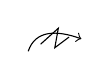
\begin{tikzpicture}[scale=.45]
\draw[->] (0,0) .. controls (.2,.6) and (.8,.6) .. (1.5,.35);
\draw (0.35,.2)--(.85,.65)--(.75,.1)--(1.15,.4);
\end{tikzpicture}}}
\margin{$\left\{\vphantom{\begin{matrix}f\\g\end{matrix}}\right.$}
\deleted{\unsure{g)}}\inserted{\unsure{f)}} Opérations de troncature, soit grossières
sur modèles, soit délicates sur $\mathcal H$.

\deleted{\unsure{h)}}\inserted{\unsure{g)}} Invariants $\pi_i$ ou $H_i$, à valeurs dans
une catégorie (souvent abélienne) associée
à la théorie.
\margin{f) et g) sont des opérations particulièrement \unsure{peu comprises}.}
\margin{\figure{\begin{tikzpicture}[scale=.4]\draw[line width=.6pt] (0,.4)--(.4,.4)--(.4,0);\end{tikzpicture}}}
